% !TeX root = main.tex

\begin{titlepage}

%%%%%%%%%%%%%%%%%%%%%%%%%%%%%%%%%%%%%%%%%%%%%%%%%%%%%%%%%%%%%%%%%%%%%%%%%%%%%%%%
%%% Strona tytułowa
%%%%%%%%%%%%%%%%%%%%%%%%%%%%%%%%%%%%%%%%%%%%%%%%%%%%%%%%%%%%%%%%%%%%%%%%%%%%%%%%

    \begin{center}
	\begin{tabular}{p{107mm} p{9cm}}
	    \begin{minipage}{9cm}
	      \begin{center}
	      Politechnika Warszawska \\
	      Wydział Elektroniki i~Technik Informacyjnych \\
	      Instytut Informatyki
	      \end{center}
	    \end{minipage}
	    &
	    \begin{minipage}{8cm}
	    \begin{flushleft}
	     \footnotesize
	      Rok akademicki 2010/2011
	    \vspace*{2.75\baselineskip}
	    \end{flushleft}
	    \end{minipage} \\
	    \vspace*{1.0\baselineskip}
	\end{tabular}
	
\includegraphics[width=4cm]{../img/logo_pw}
	\par\vspace{\smallskipamount}
	\vspace*{2\baselineskip}{\LARGE PRACA DYPLOMOWA MAGISTERSKA\par}
	\vspace{3\baselineskip}{\LARGE\strut Maciej Stefańczyk\par}
	\vspace*{2\baselineskip}{\huge\bfseries Wykorzystanie informacji z kamery 3D do nawigacji robota mobilnego\par}

	\vspace*{1\baselineskip}
	\hfill\mbox{}\par\vspace*{\baselineskip}\noindent
	\begin{tabular}[b]{@{}p{3cm}@{\ }l@{}}
	    {\large\hfill } & {\large }
	\end{tabular}
	\hfill
	\begin{tabular}[b]{@{}l@{}}
	Opiekun pracy: \\[\smallskipamount]
	{\large dr inż. Tomasz Winiarski}
	\end{tabular}\par
	\vspace*{4\baselineskip}
\begin{tabular}{p{\textwidth}}
    \begin{flushleft}
	\begin{minipage}{7cm}
	Ocena \dotfill
	\par\vspace{1.6\baselineskip}
	\dotfill
	\par\noindent
	\centerline{\footnotesize Podpis Przewodniczącego} \par
	\centerline{\footnotesize Komisji Egzaminu Dyplomowego}\par
	\end{minipage}
    \end{flushleft}
    \end{tabular}
    \end{center}

    %}

	    \cleardoublepage
%%%%%%%%%%%%%%%%%%%%%%%%%%%%%%%%%%%%%%%%%%%%%%%%%%%%%%%%%%%%%%%%%%%%%%%%%%%%%%%%
%%% Dane osobowe
%%%%%%%%%%%%%%%%%%%%%%%%%%%%%%%%%%%%%%%%%%%%%%%%%%%%%%%%%%%%%%%%%%%%%%%%%%%%%%%%
    \newpage\thispagestyle{empty}
    \begin{tabular}{p{5cm} p{11cm}}

    %%% Zdjęcie
    \begin{minipage}{5cm}
    \center
    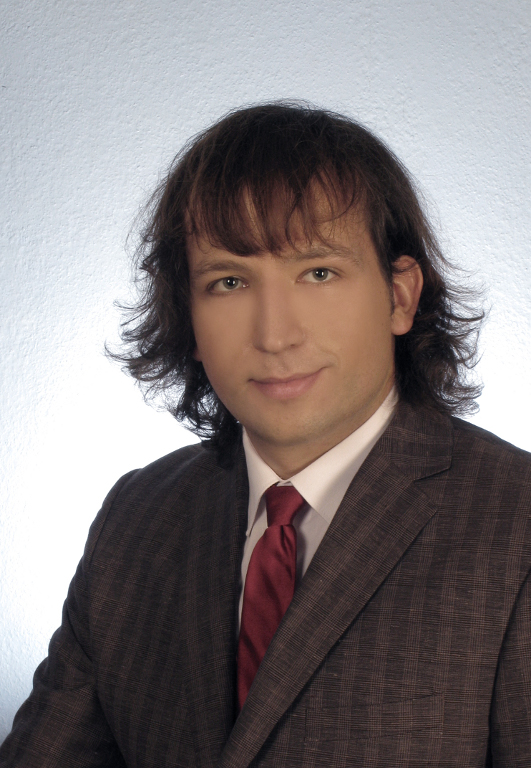
\includegraphics[height=6.5cm,width=4.5cm]{../img/foto}
    \end{minipage}
    &

    %%% Data urodzenia, specjalność itp.
    \begin{minipage}{10cm}

    Specjalność: \hfill Inżynieria Systemów Informatycznych\\
    \\
    Data urodzenia: \hfill 1985.05.04\\
    \\
    Data rozpoczęcia studiów: \hfill 2007.02.21\\

    \end{minipage}

    \end{tabular}

    \vspace*{1\baselineskip}

%%%%%%%%%%%%%%%%%%%%%%%%%%%%%%%%%%%%%%%%%%%%%%%%%%%%%%%%%%%%%%%%%%%%%%%%%%%%%%%%
%%% Życiorys
%%%%%%%%%%%%%%%%%%%%%%%%%%%%%%%%%%%%%%%%%%%%%%%%%%%%%%%%%%%%%%%%%%%%%%%%%%%%%%%%
    \begin{center}
	{\large\bfseries Życiorys}\par\bigskip
    \end{center}

    \indent
    Urodziłem się 4 maja 1985 roku w Warszawie. W~roku 2000 ukończyłem szkołę
    podstawową im.~Kornela Makuszyńskiego, a~w~latach 2000-2004 byłem uczniem
    XXVIII Liceum Ogólnokształcącego im. Jana Kochanowskiego w Warszawie.
    Po ukończeniu szkoły z~wyróżnieniem przez dwa lata studiowałem matematykę na
    wydziale Matematyki i~Nauk Informacyjnych Politechniki Warszawskiej, a~od
    21 lutego 2007 studiuję na wydziale Elektroniki i~Technik Informacyjnych tej
    samej uczelni. W dniu 29 września 2010 uzyskałem tytuł inżyniera z wynikiem
    celującym.
    \par
    \vspace{2\baselineskip}
    \hfill\parbox{15em}{{\small\dotfill}\\[-.3ex]
    \centerline{\footnotesize podpis studenta}}\par

    \vspace{3\baselineskip}

%%%%%%%%%%%%%%%%%%%%%%%%%%%%%%%%%%%%%%%%%%%%%%%%%%%%%%%%%%%%%%%%%%%%%%%%%%%%%%%%
%%% Ocena egzaminu
%%%%%%%%%%%%%%%%%%%%%%%%%%%%%%%%%%%%%%%%%%%%%%%%%%%%%%%%%%%%%%%%%%%%%%%%%%%%%%%%
    \begin{center}
 	{\large\bfseries Egzamin dyplomowy} \par\bigskip\bigskip
    \end{center}
    \par\noindent\vspace{1.5\baselineskip}
    Złożył egzamin dyplomowy w dn. \dotfill
    \par\noindent\vspace{1.5\baselineskip}
    Z wynikiem \dotfill
    \par\noindent\vspace{1.5\baselineskip}
    Ogólny wynik studiów \dotfill
    \par\noindent\vspace{1.5\baselineskip}
    Dodatkowe wnioski i uwagi Komisji \dotfill
    \par\noindent\vspace{1.5\baselineskip}
    \dotfill


	    \cleardoublepage
%%%%%%%%%%%%%%%%%%%%%%%%%%%%%%%%%%%%%%%%%%%%%%%%%%%%%%%%%%%%%%%%%%%%%%%%%%%%%%%%
%%% Streszczenie
%%%%%%%%%%%%%%%%%%%%%%%%%%%%%%%%%%%%%%%%%%%%%%%%%%%%%%%%%%%%%%%%%%%%%%%%%%%%%%%%
    \newpage\thispagestyle{empty}
    %\vspace*{2\baselineskip}
    \begin{center}
	{\large\bfseries Streszczenie}\par\bigskip
    \end{center}

    {\itshape
    Celem niniejszej pracy magisterskiej było zbadanie możliwości wykorzystania
    trójwymiarowej informacji o otoczeniu do nawigacji robota mobilnego. Dodatkowo
    należało rozważyć problem budowania trójwymiarowej mapy otoczenia oraz przedstawić
    wydajną implementację rozwiązania. Docelowy system miał pozwalać na swobodną
    nawigację robota w pomieszczeniach zamkniętych, o nieustrukturyzowanej i
    dynamicznie zmiennej konfiguracji, a także być na tyle elastyczny, aby mógł być
    zastosowany na różnych robotach przy wykorzystaniu różnego rodzaju czujników.
    Drugim zadaniem zrealizowanym w ramach pracy było przygotowanie pełnej platformy
    badawczej pozwalającej na elastyczne testowanie różnych algorytmów związanych
    z nawigacją robotów mobilnych, od przetwarzania danych sensorycznych, przez
    lokalizację i wykrywanie przeszkód aż po generowanie trajektorii.
    
    W pracy przedstawiony jest przegląd istniejących rozwiązań umożliwiających
    zbieranie informacji o otoczeniu oraz możliwych metod programowania
    robotów mobilnych. Po wyborze odpowiednich narzędzi scharakteryzowany jest 
    dokładniej wykorzystywany sprzęt oraz opisane szczegółowo stworzone poszczególne
    moduły sterowania. Praca kończy się opisem przygotowanych aplikacji testowych
    oraz podsumowaniem uzyskanych rezultatów.
    }
    \vspace*{1\baselineskip}

    \noindent{\bf Słowa kluczowe}: {\itshape YYY }
    \par
    \vspace{4\baselineskip}
    \begin{center}
	{\large\bfseries Abstract}\par\bigskip
    \end{center}
    \noindent{\bf Title}: {\itshape XXX}\par
    \vspace*{1\baselineskip}
    {\itshape

    }
    \vspace*{1\baselineskip}

    \noindent{\bf Keywords}: {\itshape XXX}

\end{titlepage}
